\subsubsection{Reinforcement Learning (RL)}

Proportional-Integral-Derivative (PID) control is widely used in control systems due to its simplicity. However, as a model-based (white-box) approach, it may exhibit limitations in highly nonlinear or complex environments, where tuning the integral component alone is often insufficient for optimal performance. In contrast, Reinforcement Learning (RL) has emerged as a data-driven (black-box) alternative for handling such complex control problems. 
To reduce the computational burden on onboard systems, reinforcement learning has increasingly been adopted as a key approach for autonomous obstacle avoidance \parencite{yu2025depth}.

The conceptual foundation of RL can be traced back to early work in artificial intelligence. Turing (1948) proposed early ideas of reward and punishment mechanisms in learning systems \parencite{barto2019rl}. Modern reinforcement learning formalizes this idea as a computational framework in which an agent learns optimal behavior through trial-and-error interactions with an environment \parencite{kaelbling1996rl}. Unlike supervised learning, RL does not rely on labeled input-output pairs. Instead, the agent receives scalar reward signals and aims to maximize cumulative long-term reward.

The mathematical foundation of RL is typically formulated using Markov Decision Processes (MDPs). In an MDP, the agent's actions influence both immediate rewards and future environmental states. As illustrated in \cref{fig:MDP}, an MDP is formally defined by four components: (1) a set of states $S$, representing all possible configurations of the environment; (2) a set of actions $A$, representing the decision space of the agent; (3) a reward function $R: S \times A \rightarrow \mathbb{R}$, which defines the immediate reward received after taking an action in a given state; and (4) a state transition function $T: S \times A \rightarrow \Delta(S)$, which defines the probability distribution over next states $s'$ given the current state $s$ and action $a$.

\begin{figure}
    \caption{Markov Decision Process diagram}\label{fig:MDP}
    \centering
    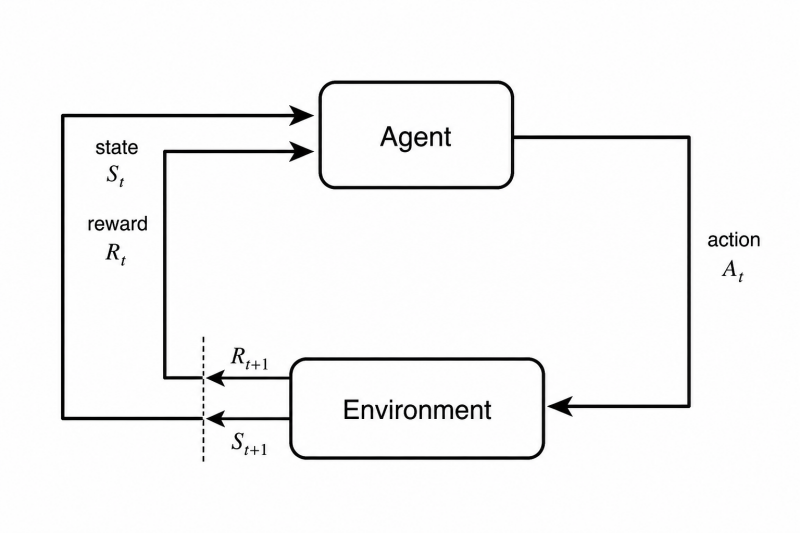
\includegraphics[width=0.8\linewidth]{img/mdp.png}
\end{figure}

In the context of training simulators, reinforcement learning provides a promising approach for developing autonomous or semi-autonomous agent behaviors that can support adaptive training environments and human-AI collaboration systems.
